\section{Introduction}
Our project is centered around the PhD research of Tim Kuipers, so you might want to expect that together we may shift more work than other group projects.

\medskip

If one wishes to print one part consisting of two incompatible materials then some interlocking geometry will need to be introduced at the interface between these two materials in order to make these two materials adhere to each other mechanically.
We consider two materials, a hard one (shown in green) and a soft one (in cyan), which are placed next to each other such that the interface is horizontal
and we will consider a tensile for is applied orthogonal to the interface.

The structure consists of parallel beams of alternating materials in some layers, and in other layers the beams of both materials are rotated, so that they connect the various beams of the former, thusly interlocking the materials.
We want to optimize the structure such that it can withstand the highest tensile force, for an arbitrarily large interface;
that is, we want to optimize the effective ultimate tensile strength of the interlocking micro-structure.
We want to optimize our structure such that none of the components of breaks or yields at the highest applied force.
On the other hand we would like our structure to be as small as possible, which is captured in both constraints and objective functions.

We consider two closely related interlocking geometries consisting of beams of either material connected 
Both of these geometries are limited by manufacturing constraints:
\begin{itemize}
	\item heights are a discrete multiple of the layer thickness $h_\text{min}$
	\item widths are continuous, but at least twice the nozzle size $w_\text{min}$
	\item the width of a very long beam may be smaller: at least once the nozzle size $w_\text{min}$
\end{itemize}


We consider two orientations of the interlocking pattern:
\begin{description}
	\item[Straight] even beams (`cross beams') are aligned parallel to the interface and odd beams (`fingers') are perpendicular
	\item[Diagonal] even beams and odd beams (both `fingers') are at equal and opposite angles w.r.t. the interface.
\end{description}






\section{Straight Orientation}



\begin{figure}
	\centering
	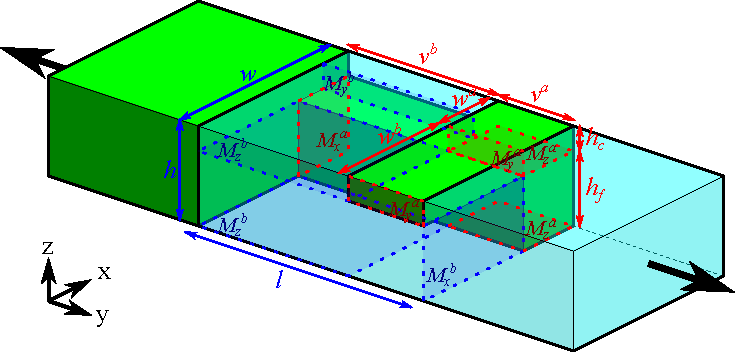
\includegraphics[width=\columnwidth]{sources/method/straight_model_v3.pdf}
	\caption{
		One straight unit cell connecting material $a$ (left) to material $b$ (right).
		Failure can happen along the fingers ($M_x$), along the cross beams ($M_y$) or at the interface between the two ($M_z$) for either material.}
	\label{fig:failure_modes}
\end{figure}

\Cref{fig:failure_modes} shows one cell of the straight structure, along with the design variables and the failure modes.
The optimization then consists of the following:

\begin{align}
	& \max \frac{F}{\left( w^a + w^b \right) \left( h_\text{f} + h_\text{c} \right) } \\
	& \min h_\text{f} h_\text{c} \\
	\text{subject to} & \nonumber \\
	w^m &\ge w_\text{min}^m \\
	v^m &\ge v_\text{min}^m \\
	h_\text{f} &\ge h_\text{min} \\
	h_\text{c} &\ge h_\text{min} \\
	v^a + v^b &\le v_\text{max} \\
	\frac{ F }{ w^m h_\text{f} } &\le \sigma^m_\text{yield} &&\text{ failure mode } M_x^m \\
	\frac{ 2 F }{ 3 v^m h_\text{c}} &\le \tau^m 			&&\text{ failure mode } M_y^m \\
	\frac{ 2 F }{ 3 v^m w^m } &\le \tau^m_\text{Z} 			&&\text{ failure mode } M_z^m \\
	& \text{for both materials } && m \in \{a, b\} \nonumber
\end{align}

\iffalse

\paragraph{Monotonicity Analysis}
\begin{align*}
	\min & 1 - \frac{F}{\left( w^a + w^b \right) \left( h_\text{f} + h_\text{c} \right) }
																		&& F^-, w^{a+}, w^{b+},  h_\text{f}^+, h_\text{c}^+\\
	\text{subject to} & \nonumber \\
	1 - \frac{w^m }{w_\text{min}^m} &\le 0    							&& w^{m-} \\
	1 - \frac{v^m }{w_\text{min}^m} &\le 0    							&& v^{m-} \\
	1 - \frac{h_\text{f}}{h_\text{min}} &\le 0 							&& h_\text{f}^- \\
	1 - \frac{h_\text{c}}{h_\text{min}} &\le 0 							&& h_\text{c}^- \\
	\frac{v^a + v^b}{ v_\text{max} }  - 1&\le 0 						&& v^{a+}, v^{b+} \\
	\frac{ F }{ w^m h_\text{f} \sigma^m_\text{yield} } - 1&\le 0 		&& F^+, w^{m-}, h_\text{f}^- \\
	\frac{ 2 F }{ 3 v^m h_\text{c} \tau^m } - 1 &\le 0 					&& F^+, v^{m-}, h_\text{c}^- \\
	\frac{ 2 F }{ 3 v^m w^m \tau^m_\text{Z} } - 1 &\le 0 					&& F^+, v^{m-}, w^{m-} \\
	\nonumber \\
	F^m &= \sigma^m w^m h_\text{f} \\
	\dots \\
	& \text{for both materials } m \in \{a, b\}
\end{align*}
\fi


This looks like a multi-objective optimization problem, but without the second objective the problem is under-constrained.
Adding the second objective actually means there's one unique solution - rather counter-intuitively.

The $v^m$ variables don't figure in the objective, but they do appear in the constraints and therefore are also subject to the optimization.

We should be able to find analytical solution(s), depending on the size of $v_\text{max}$ w.r.t. the other constraints.

Possible extensions:
\begin{itemize}
	\item Take bending stress constraint into account.
	\item Consider multiple repetitions of the cell in the loading direction.
	\item Consider tensile load in Z direction.
	\item Consider FEM model.
\end{itemize}

\iffalse
Formula is given by this? :
% from https://skyciv.com/docs/tutorials/beam-tutorials/bending-moment-equations/
\begin{align*}
	\sigma_\text{bend} &= \frac{M r}{I} \\
	&= \frac{M \nicefrac12 v}{I} \\
	M_\text{max} &= \frac{v L}{12} \text{ for distributed force and fixed sides} 
\end{align*}
\fi













\section{Slanted design}

\begin{figure}
	\centering
	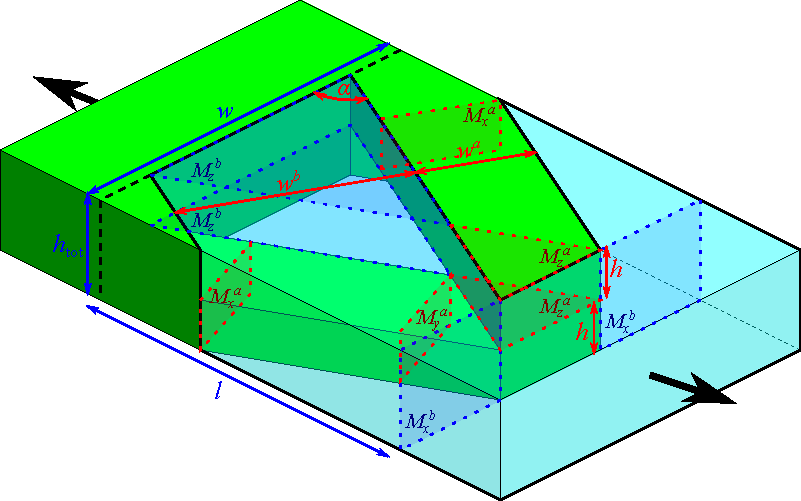
\includegraphics[width=\columnwidth]{sources/method/diagonal_model_v3.pdf}
	\caption{
		One diagonal unit cell connecting material $a$ (left) to material $b$ (right).
		Failure can happen along both the fingers ($M_x$), twice along one finger ($M_y$) or at the interface between the two fingers ($M_z$) for either material.}
	\label{fig:diagonal_model}
\end{figure}

TODO: \cref{fig:diagonal_model}
